%\documentclass[fleqn]{book}
\documentclass[11pt]{amsbook}

\usepackage[turkish]{babel}

%\usepackage{../HBSuerDemir}	% ------------------------
\usepackage{../Ceyhun}	% ------------------------
\usepackage{../amsTurkish}


\begin{document}
\setcounter{page}{210}
\setcounter{section}{3}


\renewcommand{\theenumi}{\alph{enumi}}
\section{Düzlemsellik}
\setcounter{subsection}{2}
\subsection{Çifteşlik}
\begin{enumerate}
	\item $Ç_1$ çizgesini düzleme çiz,
	\item Her tüzü (dış yüzü de) bir düğüm ile belirle,
	\item Eğer $a_0$ ayrıtı, $y_1$ ve $y_2$ yüzlerini ayırıyorsa, bu yüzleri belirleyen $d_1^{\prime}$ ve $d_2^{\prime}$ düğümlerini $a_0^{\prime}$ ayrıtı ile bitiştir, 
	\item (c) de açıklanan işlemi, çizgedeki bütün \\
% ++++++++++++++++++++++++++++++++++++++
\hPage{210}
% ++++++++++++++++++++++++++++++++++++++
		ayrıtlar için yinele,
	\item $a_i^{\prime}$ ayrıtları, $d_i^{\prime}$ düğümleri ile birlikte, $Ç_1$ in çifteşi $Ç_2$ çizgesini tanımlayacaktır.
\end{enumerate}

Şekil \ref{sekil1} de, bu yönteme göre düzlemsel bir çizgenin çifteşinin elde edilmesi gösterilmiştir. 
\setcounter{figure}{1}
\begin{figure}[htb]
	\centering
	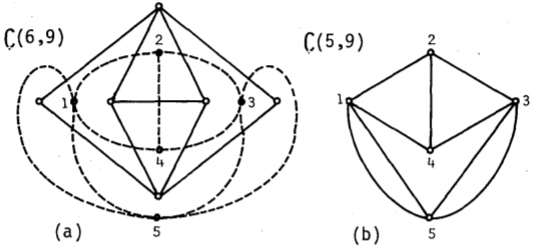
\includegraphics[width=0.45\textwidth]{images/ceyhun-210-fig01}
	\caption{Ç(6,9) çizgesinde, çifteş çizge Ç(5,9) un elde edilmesi.}
	\label{sekil1}
\end{figure}

İlkel bir durum olarak, tekayrıtın çifteşinin 
tekçevre ya da tekçevrenin çifteşinin tekayrıt ve
tekdüğümün çifteşinin yine tekdüğüm olduğu
gösterilebilir. Çifteşi kendisine eşbiçimli olan
çizgelere, \textit{özçifteş} çizge diyeceğiz. Şekil
\ref{sekil2} de, özçifteş bir çizge gösterilmiştir
(özçifteş çizgeye başka bir örnek daha bulunuz).
Özçifteşlik ve ilişkin özellikleri, çizge kuramında
açık sorunlarla dolu bir konudur ve üzerinde daha
çok durmayacağız. 

% ++++++++++++++++++++++++++++++++++++++
\hPage{211}
% ++++++++++++++++++++++++++++++++++++++

\begin{figure}[htb]
	\centering
	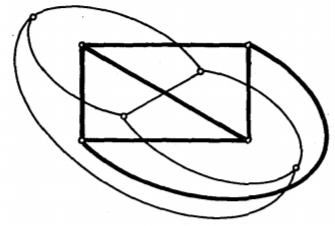
\includegraphics[width=0.45\textwidth]{images/ceyhun-210-fig02}
	\caption{Özçifteş çizgeye örnek.}
	\label{sekil2}
\end{figure}

\end{document}